\documentclass[11pt]{article}

\usepackage[margin=1in]{geometry}
\usepackage{amsmath,amssymb,mathtools}
\usepackage{booktabs}
\usepackage{array}
\usepackage{xcolor}
\usepackage{hyperref}
\usepackage{enumitem}
\usepackage{listings}
\usepackage{tikz}
\usetikzlibrary{arrows.meta,positioning,fit,calc,shapes.geometric}

\hypersetup{
  colorlinks=true,
  linkcolor=blue!60!black,
  urlcolor=blue!60!black,
  citecolor=blue!60!black
}

\definecolor{mfblue}{RGB}{38,91,160}
\definecolor{mfgreen}{RGB}{46,125,50}
\definecolor{mforange}{RGB}{198,117,34}
\definecolor{mfpurple}{RGB}{110,67,153}
\definecolor{mfgrey}{RGB}{245,246,248}

\lstdefinestyle{matterformer}{
  basicstyle=\ttfamily\small,
  backgroundcolor=\color{mfgrey},
  frame=single,
  rulecolor=\color{black!15},
  breaklines=true,
  columns=fullflexible,
  keepspaces=true
}
\lstset{style=matterformer}

\title{\textbf{Modular Matterformer Hybrid Stack}\\
\large Architecture, Streams, Schedules, Options, and Equations}
\author{Matterformer}
\date{\today}

\begin{document}
\maketitle

\begin{abstract}
This note describes the hybrid Matterformer stack implemented on the
\texttt{modular-matterformer} branch.  The stack combines three reusable layer
families: local compact kNN simplicial layers, global tetrahedral Platonic
layers, and global scalar Transformer layers.  A macro-block scheduler expands
simple count configurations such as \texttt{[2,1,0]} into executable layer
orders.  The implementation is additive: the old dense simplicial and MHA
trunks remain available, and \texttt{attn\_type="hybrid"} selects the new path.
\end{abstract}

\tableofcontents
\newpage

\section{High-Level Picture}

The hybrid trunk keeps two feature streams:

\begin{itemize}[leftmargin=1.5em]
  \item \textbf{Scalar stream}: ordinary atom/token features
  \[
    h_i \in \mathbb{R}^{C_s}.
  \]
  In the current EDM wrappers, \texttt{d\_model} is this scalar width.

  \item \textbf{Tetra group stream}: features over a finite tetrahedral group
  \[
    F_i(g) \in \mathbb{R}^{C_g},
    \qquad g \in G_{\mathrm{tet}},
    \qquad |G_{\mathrm{tet}}|=12.
  \]
  The effective group width is \(12 C_g\).
\end{itemize}

The scalar stream is always the output stream consumed by existing QM9, GEOM
Drugs, and MOF heads.  The group stream is optional and is introduced when the
schedule contains tetra layers or when \texttt{branch\_mode} requests it.

\begin{figure}[h]
\centering
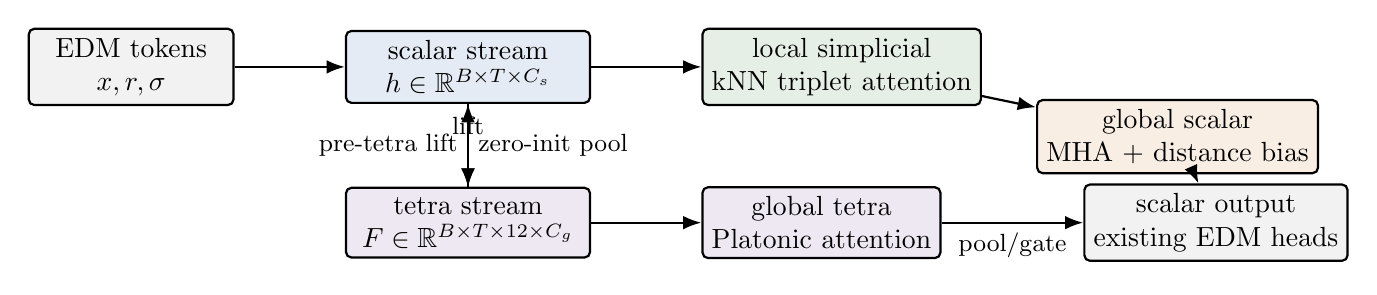
\begin{tikzpicture}[
  node distance=1.05cm and 1.4cm,
  box/.style={draw, rounded corners=2pt, thick, align=center, minimum width=2.6cm, minimum height=0.78cm},
  stream/.style={draw, rounded corners=2pt, thick, align=center, minimum width=3.1cm, minimum height=0.78cm},
  arrow/.style={-Latex, thick}
]
  \node[box, fill=black!5] (input) {EDM tokens\\ \(x, r, \sigma\)};
  \node[stream, fill=mfblue!12, right=of input] (scalar) {scalar stream\\ \(h \in \mathbb{R}^{B\times T\times C_s}\)};
  \node[stream, fill=mfpurple!12, below=of scalar] (group) {tetra stream\\ \(F \in \mathbb{R}^{B\times T\times 12\times C_g}\)};
  \node[box, fill=mfgreen!12, right=of scalar] (simp) {local simplicial\\ kNN triplet attention};
  \node[box, fill=mfpurple!12, right=of group] (tetra) {global tetra\\ Platonic attention};
  \node[box, fill=mforange!12, above right=0.15cm and 1.2cm of tetra] (trivial) {global scalar\\ MHA + distance bias};
  \node[box, fill=black!5, right=1.8cm of tetra] (out) {scalar output\\ existing EDM heads};

  \draw[arrow] (input) -- (scalar);
  \draw[arrow] (scalar) -- node[above, font=\small] {lift} (group);
  \draw[arrow] (scalar) -- (simp);
  \draw[arrow] (simp) -- (trivial);
  \draw[arrow] (group) -- (tetra);
  \draw[arrow] (tetra) -- node[below, font=\small] {pool/gate} (out);
  \draw[arrow] (trivial) -- (out);
  \draw[arrow, dashed] (scalar) -- node[left, font=\small] {pre-tetra lift} (group);
  \draw[arrow, dashed] (group) -- node[right, font=\small] {zero-init pool} (scalar);
\end{tikzpicture}
\caption{Hybrid Matterformer streams and layer families.}
\end{figure}

\section{Core State Object}

Internally, the trunk can be described by a state object:

\[
\mathcal{S}
=
\left(
  r,\; m,\; h,\; F,\; \mathcal{G},\; c,\; \sigma
\right),
\]

where:

\begin{center}
\begin{tabular}{lll}
\toprule
Symbol & Tensor shape & Meaning \\
\midrule
\(r\) & \(B\times N\times 3\) & coordinates for atom/block tokens \\
\(m\) & \(B\times T\) & padding mask, true for padded tokens \\
\(h\) & \(B\times T\times C_s\) & scalar token stream \\
\(F\) & \(B\times T\times G\times C_g\) & group stream, \(G=12\) for tetra \\
\(\mathcal{G}\) & cache & dense geometry plus compact kNN geometry \\
\(c\) & \(B\times C_s\) or null & AdaLN/noise conditioning embedding \\
\(\sigma\) & \(B\) or null & EDM noise level for geometry gates \\
\bottomrule
\end{tabular}
\end{center}

Current wrapper convention:

\[
  C_s = \texttt{d\_model}.
\]

The group width is configured separately:

\[
  C_g = \texttt{tetra\_dim\_per\_frame},
  \qquad
  d_{\mathrm{group}} = 12 C_g.
\]

\section{Macro-Block Scheduler}

Each macro-block contains a count of three layer types:

\[
\texttt{block\_mix}
=
[n_S,n_T,n_I],
\]

where:

\begin{itemize}[leftmargin=1.5em]
  \item \(S\): local compact kNN simplicial layer.
  \item \(T\): global tetrahedral Platonic layer.
  \item \(I\): global trivial or invariant scalar Transformer layer.
\end{itemize}

For example:

\begin{lstlisting}[language=Python]
num_blocks = 4
block_mix = [[2, 1, 0], [2, 0, 1]]
order_policy = "local_then_global"
\end{lstlisting}

expands round-robin to:

\[
\begin{aligned}
B_0 &= [S,S,T],\\
B_1 &= [S,S,I],\\
B_2 &= [S,S,T],\\
B_3 &= [S,S,I].
\end{aligned}
\]

\begin{figure}[h]
\centering
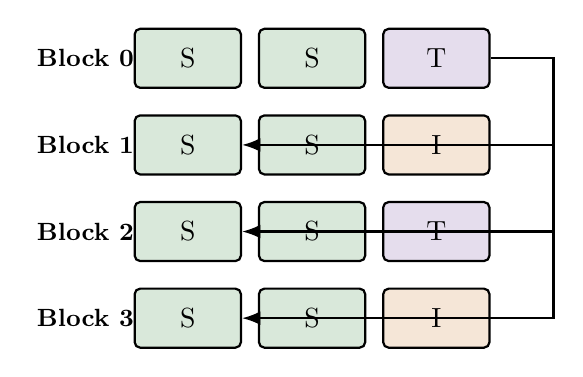
\begin{tikzpicture}[
  layer/.style={draw, rounded corners=2pt, thick, minimum width=1.35cm, minimum height=0.75cm, align=center},
  arrow/.style={-Latex, thick},
  blocklabel/.style={font=\small\bfseries}
]
  \node[blocklabel] at (-1.3,0) {Block 0};
  \node[layer, fill=mfgreen!18] (s00) at (0,0) {S};
  \node[layer, fill=mfgreen!18, right=0.2cm of s00] (s01) {S};
  \node[layer, fill=mfpurple!18, right=0.2cm of s01] (t0) {T};

  \node[blocklabel] at (-1.3,-1.1) {Block 1};
  \node[layer, fill=mfgreen!18] (s10) at (0,-1.1) {S};
  \node[layer, fill=mfgreen!18, right=0.2cm of s10] (s11) {S};
  \node[layer, fill=mforange!18, right=0.2cm of s11] (i1) {I};

  \node[blocklabel] at (-1.3,-2.2) {Block 2};
  \node[layer, fill=mfgreen!18] (s20) at (0,-2.2) {S};
  \node[layer, fill=mfgreen!18, right=0.2cm of s20] (s21) {S};
  \node[layer, fill=mfpurple!18, right=0.2cm of s21] (t2) {T};

  \node[blocklabel] at (-1.3,-3.3) {Block 3};
  \node[layer, fill=mfgreen!18] (s30) at (0,-3.3) {S};
  \node[layer, fill=mfgreen!18, right=0.2cm of s30] (s31) {S};
  \node[layer, fill=mforange!18, right=0.2cm of s31] (i3) {I};

  \draw[arrow] (t0.east) -- ++(0.8,0) |- (s10.east);
  \draw[arrow] (i1.east) -- ++(0.8,0) |- (s20.east);
  \draw[arrow] (t2.east) -- ++(0.8,0) |- (s30.east);
\end{tikzpicture}
\caption{Recommended hybrid v1 schedule: local layers dominate, with alternating tetra and scalar global layers.}
\end{figure}

\subsection{Order Policies}

\begin{center}
\begin{tabular}{p{0.28\linewidth}p{0.58\linewidth}}
\toprule
Policy & Behavior \\
\midrule
\texttt{local\_then\_global} &
Runs all \(S\) layers first, then all \(T\) layers, then all \(I\) layers inside each macro-block. \\
\texttt{interleave} &
Distributes global layers between local layers.  Useful when global context should refresh local features more often. \\
\texttt{explicit} &
Uses explicit layer type lists.  This is best for exact ablations and checkpoint reproducibility. \\
\bottomrule
\end{tabular}
\end{center}

\section{Geometry Cache and Local kNN}

The local path builds compact neighbor tensors from the existing dense geometry
adapter.  For each query atom \(i\), keep a fixed-size neighbor set
\[
  \mathcal{N}_K(i)
  =
  \operatorname{kNN}(i),
  \qquad
  |\mathcal{N}_K(i)| \le K.
\]

For \(j \in \mathcal{N}_K(i)\):

\[
  r_{ij} = x_j - x_i,
  \qquad
  d_{ij} = \|r_{ij}\|_2,
  \qquad
  \hat r_{ij} = \frac{r_{ij}}{d_{ij}+\epsilon}.
\]

The compact cache has the operational shape:

\begin{center}
\begin{tabular}{lll}
\toprule
Name & Shape & Meaning \\
\midrule
\texttt{neighbor\_idx} & \(B\times N\times K\) & neighbor indices \\
\texttt{neighbor\_mask} & \(B\times N\times K\) & valid neighbor flags \\
\texttt{rel} & \(B\times N\times K\times 3\) & relative vectors \(x_j-x_i\) \\
\texttt{dist} & \(B\times N\times K\) & neighbor distances \\
\texttt{unit} & \(B\times N\times K\times 3\) & unit directions \\
\texttt{rbf} & \(B\times N\times K\times R_{\mathrm{rbf}}\) & radial basis \\
\texttt{pair\_mask} & \(B\times N\times K\times K\) & valid neighbor pair flags \\
\bottomrule
\end{tabular}
\end{center}

For periodic MOF Stage1 data, these tensors are derived from the existing
periodic minimal-image geometry adapter, so the local kNN graph respects the
periodic distance convention already used by Matterformer.

\section{Local Simplicial Layer}

The local simplicial layer updates the scalar stream for coordinate-backed atom
tokens.  Extra global tokens, such as the MOF lattice token, pass through local
layers and are updated by global layers.

\subsection{Projected Features}

For each head \(a\), project scalar atom features into five tensors:

\[
  q_i^a,\; k_{1,j}^a,\; v_{1,j}^a,\; k_{2,k}^a,\; v_{2,k}^a
  \in \mathbb{R}^{D_h}.
\]

The triadic content score is:

\[
  C^a_{i,j,k}
  =
  \sum_{d=1}^{D_h}
  q^a_{i,d}
  k^a_{1,j,d}
  k^a_{2,k,d}.
\]

\subsection{Compact Bias}

The compact branch now keeps the scalar local bias rotation invariant.  Radial
MLPs see scalar distance features only:

\[
  e_{ij}
  =
  \operatorname{RBF}(d_{ij}),
\]

then produce scalar coefficients:

\[
  u^a_{ij},\quad v^a_{ik},\quad
  a^a_{ij,\ell,t},\quad b^a_{ij,\ell,t}.
\]

The coefficients are multiplied by fixed spherical/STF basis blocks
\[
  \Phi_0(\hat r)\in\mathbb{R}^{1},
  \qquad
  \Phi_1(\hat r)\in\mathbb{R}^{3},
  \qquad
  \Phi_2(\hat r)\in\mathbb{R}^{5}.
\]

Thus:

\[
  L^a_{ij}
  =
  \operatorname{concat}_{\ell,t}
  a^a_{ij,\ell,t}\Phi_\ell(\hat r_{ij}),
  \qquad
  R^a_{ik}
  =
  \operatorname{concat}_{\ell,t}
  b^a_{ik,\ell,t}\Phi_\ell(\hat r_{ik}).
\]

The low-rank angle term is:

\[
  A^a_{i,j,k}
  =
  \frac{1}{\sqrt{R}}
  \langle L^a_{ij}, R^a_{ik}\rangle.
\]

Because the dot product pairs basis blocks of the same degree, this term is a
learned Legendre/spherical filter over the angle
\(\hat r_{ij}\cdot\hat r_{ik}\), not an arbitrary global-coordinate MLP.

The full score is:

\[
  S^a_{i,j,k}
  =
  C^a_{i,j,k}
  +
  \gamma^a_i
  \left(u^a_{ij}+v^a_{ik}\right)
  +
  \eta^a_i A^a_{i,j,k}.
\]

The logit gates \(\gamma\) and \(\eta\) are initialized at zero, so the score
starts close to pure content attention.

\subsection{Attention and Output}

The attention distribution is normalized over neighbor pairs:

\[
  p^a_{i,j,k}
  =
  \frac{\exp(S^a_{i,j,k})}
  {\sum_{j'\in\mathcal{N}_K(i)}
   \sum_{k'\in\mathcal{N}_K(i)}
   \exp(S^a_{i,j',k'})}.
\]

The value output is:

\[
  o_i^a
  =
  \sum_{j,k\in\mathcal{N}_K(i)}
  p^a_{i,j,k}
  \left(
    v^a_{1,j}\odot v^a_{2,k}
  \right).
\]

If value-side message residuals are enabled, the extra message coefficient is:

\[
  m^a_{i,r}
  =
  \frac{1}{\sqrt{R_m}}
  \sum_{j,k}
  p^a_{i,j,k}
  M^{L,a}_{ijr}
  M^{R,a}_{ikr},
\]

and the output receives:

\[
  \Delta o^a_i
  =
  \sum_{r=1}^{R_m}m^a_{i,r}B^a_{r}.
\]

By default, \texttt{message.enabled = False}.

\subsection{Complexity}

For batch size \(B\), atoms \(N\), heads \(H\), neighbors \(K\), head width
\(D_h\), and low-rank geometry width \(R\):

\[
  \mathcal{O}\left(B H N K^2(D_h+R)\right).
\]

This is the intended scalable replacement for dense \(N^2\) simplicial tensors.

\section{Tetra Platonic Global Layer}

The tetra layer updates only the group stream:

\[
  F_i(g)\in\mathbb{R}^{C_g},
  \qquad g\in G_{\mathrm{tet}},
  \qquad |G_{\mathrm{tet}}|=12.
\]

It uses group-constrained linear maps.  The flattened storage shape is
\(G C_g\), but the linear map is not an arbitrary dense \(\mathbb{R}^{GC_g}\)
linear layer.  Instead, it is a group convolution:

\[
  Y_h
  =
  \sum_{g\in G}
  W_{g^{-1}h}X_g.
\]

This weight tying ensures finite-group equivariance:

\[
  \mathcal{L}(\rho(a)X)
  =
  \rho(a)\mathcal{L}(X),
  \qquad a\in G_{\mathrm{tet}}.
\]

\subsection{Group RoPE Attention}

For each group frame \(g\), the RoPE frequencies are rotated by the group
matrix \(R_g\).  The phase is:

\[
  \theta_{i,g,h,f}
  =
  x_i^\top
  R_g\omega_{h,f}.
\]

Then queries and keys are rotated with the usual two-channel RoPE operation.
The current dense implementation uses standard scaled dot-product attention over
the combined group-head axis.

\[
  \operatorname{Attn}(Q,K,V)
  =
  \operatorname{softmax}
  \left(
    \frac{QK^\top}{\sqrt{D_h}}
  \right)V.
\]

When \texttt{rope\_on\_values=True}, values are rotated before attention and
the output is inverse-rotated afterward.

\section{Trivial Global Layer}

The trivial global layer updates the scalar stream using the existing
Matterformer MHA block.  It now exposes explicit geometry modes.  The strict
scalar mode is distance-bias attention:

\[
  S_{ij}^{a}
  =
  (q_i^a)^\top k_j^a
  +
  b^a(d_{ij}, \text{edge features}).
\]

For QM9 EDM direct-coordinate experiments, the performance mode is:

\[
  \texttt{edge\_delta\_bias},
\]

which uses distance features plus raw relative coordinate vectors
\(\Delta x_{ij}\) in the existing \texttt{GeometryBiasBuilder}.  This is not a
strict rotation-invariant scalar path, but it matches the old active MHA
geometry-bias behavior used by the successful scalar SIT run.

\texttt{distance\_bias} means distance-only.  \texttt{none} disables scalar
global geometry bias.

\section{Scalar--Group Coupling}

The scalar stream and tetra stream are coupled around tetra layers.  The
important operational order is:

\[
  \text{current scalar}
  \xrightarrow{\text{pre lift}}
  \text{group}
  \xrightarrow{\text{tetra}}
  \text{group}
  \xrightarrow{\text{zero-init post pool}}
  \text{scalar}.
\]

This avoids running tetra on a stale group stream.  The scalar-to-group pre
gate can start open, while the group-to-scalar residual gate starts at zero so
the scalar path remains stable at initialization.

\subsection{Scalar to Group}

The scalar-to-group pre-lift is copied to all frames:

\[
  \Delta F_i(g)
  =
  \alpha
  W_{\mathrm{s2g}}h_i,
  \qquad
  \forall g\in G.
\]

Since the lifted value is identical over \(g\), it does not introduce a
frame-specific orientation.

\subsection{Group to Scalar}

The group stream is mean-pooled:

\[
  \bar F_i
  =
  \frac{1}{|G|}
  \sum_{g\in G}F_i(g),
\]

then projected into scalar channels:

\[
  \Delta h_i
  =
  \beta
  W_{\mathrm{g2s}}\bar F_i.
\]

For QM9 sidecar runs, \(\alpha\) starts at \(1.0\) for the pre-tetra lift and
\(\beta\) starts at \(0.0\) for the post-tetra scalar residual.

\section{Configuration Surface}

\subsection{Top-Level Hybrid Config}

\begin{center}
\begin{tabular}{p{0.29\linewidth}p{0.56\linewidth}}
\toprule
Field & Meaning \\
\midrule
\texttt{num\_blocks} & Number of macro-blocks. \\
\texttt{block\_mix} & Either one \([n_S,n_T,n_I]\) mix or a list of mixes repeated round-robin. \\
\texttt{order\_policy} & \texttt{local\_then\_global}, \texttt{interleave}, or \texttt{explicit}. \\
\texttt{explicit\_orders} & Exact layer orders when \texttt{order\_policy="explicit"}. \\
\texttt{branch\_mode} & \texttt{auto}, \texttt{scalar\_only}, \texttt{tetra\_only}, or \texttt{two\_stream}. \\
\texttt{scalar\_dim} & Must equal \texttt{d\_model} in current EDM wrappers. \\
\texttt{tetra\_dim\_per\_frame} & Channels per tetra frame. Effective group width is \(12C_g\). \\
\texttt{simplicial} & Local compact simplicial layer config. \\
\texttt{tetra} & Global Platonic layer config. \\
\texttt{trivial} & Global scalar MHA config. \\
\texttt{coupling} & Scalar--group coupling config. \\
\bottomrule
\end{tabular}
\end{center}

\subsection{Simplicial Options}

\begin{center}
\begin{tabular}{p{0.29\linewidth}p{0.56\linewidth}}
\toprule
Field & Meaning \\
\midrule
\texttt{target} & Current safe default is \texttt{scalar}. \\
\texttt{k\_neighbors} & Local neighbor cap \(K\), default 32. \\
\texttt{num\_heads} & Simplicial attention heads. Defaults to model \texttt{n\_heads}. \\
\texttt{head\_dim} & Optional head width. If null, uses \(\texttt{d\_model}/\texttt{num\_heads}\). \\
\texttt{bias.angle\_rank} & Low-rank angle width \(R\). \\
\texttt{bias.radial\_basis\_dim} & RBF width for compact edge features. \\
\texttt{bias.radial\_cutoff} & Optional RBF cutoff. \\
\texttt{message.enabled} & Enables value-side low-rank message residual. Default false. \\
\texttt{message.rank} & Message residual rank. \\
\texttt{kernel.backend} & \texttt{triton\_knn} or \texttt{torch}. On CUDA with Triton installed, \texttt{triton\_knn} uses the compact kNN simplicial attention kernel; unsupported cases fall back to the reference path. \\
\bottomrule
\end{tabular}
\end{center}

\subsection{Tetra Options}

\begin{center}
\begin{tabular}{p{0.29\linewidth}p{0.56\linewidth}}
\toprule
Field & Meaning \\
\midrule
\texttt{group} & \texttt{tetrahedron}. \\
\texttt{group\_order} & Must be 12 for tetra. \\
\texttt{heads\_per\_frame} & Base attention heads per group frame. \\
\texttt{rope\_sigma} & Initial RoPE frequency scale. \\
\texttt{learned\_freqs} & Whether RoPE frequencies are trainable. \\
\texttt{use\_key} & If false, Platonic attention uses all-ones positional keys. \\
\texttt{rope\_on\_values} & Rotate values and inverse-rotate outputs. \\
\texttt{ffn\_mult} & Group-equivariant FFN expansion factor. \\
\bottomrule
\end{tabular}
\end{center}

\subsection{Trivial Options}

\begin{center}
\begin{tabular}{p{0.29\linewidth}p{0.56\linewidth}}
\toprule
Field & Meaning \\
\midrule
\texttt{target} & Current default is \texttt{scalar}. \\
\texttt{attention.kind} & \texttt{mha}. \\
\texttt{attention.num\_heads} & Scalar MHA head count. \\
\texttt{attention.position\_encoding} & Recommended default is \texttt{distance\_bias}. \\
\texttt{ffn.ffn\_mult} & Scalar FFN expansion factor. \\
\bottomrule
\end{tabular}
\end{center}

\section{Recommended QM9 EDM Hybrid Configuration}

For QM9 EDM, the current recommended SIT sidecar configuration keeps one local
simplicial layer per macro-block, makes scalar all-to-all attention the main
long-range path, and uses tetra global attention as a narrow sidecar:

\begin{lstlisting}[language=Python]
hybrid_config = {
    "num_blocks": 8,
    "block_mix": [
        [1, 0, 1],  # S, scalar global
        [1, 0, 1],  # S, scalar global
        [1, 1, 0],  # S, tetra global
        [1, 0, 1],  # S, scalar global
    ],
    "order_policy": "local_then_global",
    "branch_mode": "two_stream",

    # Current wrapper rule: scalar_dim must match d_model.
    "scalar_dim": 768,

    # 12 tetra frames * 32 channels = 384 effective sidecar width.
    "tetra_dim_per_frame": 32,

    "simplicial": {
        "target": "scalar",
        "k_neighbors": 32,
        "num_heads": 12,
        "head_dim": None,
        "bias": {
            "kind": "spherical_low_rank",
            "angle_rank": 32,
            "channels_by_l": {0: 5, 1: 4, 2: 3},
            "radial_basis_dim": 32,
            "radial_cutoff": None,
        },
        "message": {
            "enabled": False,
            "rank": 16,
        },
        "kernel": {
            "backend": "triton_knn",
        },
    },

    "tetra": {
        "group": "tetrahedron",
        "group_order": 12,
        "heads_per_frame": 2,
        "rope_sigma": 4.0,
        "learned_freqs": True,
        "use_key": False,
        "rope_on_values": True,
        "ffn_mult": 4,
    },

    "trivial": {
        "target": "scalar",
        "attention": {
            "kind": "mha",
            "num_heads": 12,
            "position_encoding": "edge_delta_bias",
        },
        "ffn": {
            "ffn_mult": 4,
        },
    },

    "coupling": {
        "init_group_from_scalar": True,
        "scalar_to_group": {
            "enabled": True,
            "pre_gate_init": 1.0,
            "gate_init": 0.0,
        },
        "group_to_scalar": {
            "enabled": True,
            "gate_init": 0.0,
        },
        "after_each_tetra": True,
        "after_each_macro_block": False,
    },
}
\end{lstlisting}

The corresponding Python construction is:

\begin{lstlisting}[language=Python]
from matterformer.models import QM9EDMModel

model = QM9EDMModel(
    atom_channels=6,
    d_model=768,
    n_heads=12,
    n_layers=8,
    attn_type="hybrid",
    hybrid_config=hybrid_config,
)
\end{lstlisting}

The current training CLI can activate the default hybrid config directly:

\begin{lstlisting}[language=bash]
PYTHONPATH=src python scripts/train_qm9_edm.py \
  --data-dir ./data/qm9 \
  --attn-type hybrid \
  --hybrid-config-json configs/qm9_hybrid/sit_sidecar_additive_narrow_960eff.json \
  --d-model 768 \
  --n-heads 12 \
  --n-layers 8 \
  --batch-size 64 \
  --coord-embed-mode none \
  --noise-conditioning concat
\end{lstlisting}

The CLI accepts a nested hybrid JSON object through
\texttt{--hybrid-config-json}.  The current launcher scripts use this path for
reproducible Slurm experiments.

\section{Ablation Configurations}

\subsection{Pure Local Simplicial}

\begin{lstlisting}[language=Python]
hybrid_config = {
    "num_blocks": 10,
    "block_mix": [1, 0, 0],
    "branch_mode": "scalar_only",
    "simplicial": {
        "target": "scalar",
        "k_neighbors": 32,
        "bias": {"angle_rank": 32, "radial_basis_dim": 32},
        "message": {"enabled": False},
        "kernel": {"backend": "triton_knn"},
    },
}
\end{lstlisting}

\subsection{Pure Tetra Global}

\begin{lstlisting}[language=Python]
hybrid_config = {
    "num_blocks": 10,
    "block_mix": [0, 1, 0],
    "branch_mode": "tetra_only",
    "tetra_dim_per_frame": 32,
    "tetra": {
        "group": "tetrahedron",
        "group_order": 12,
        "heads_per_frame": 1,
        "rope_sigma": 0.5,
        "learned_freqs": True,
        "use_key": False,
        "rope_on_values": True,
    },
}
\end{lstlisting}

\subsection{Pure Scalar Global Transformer}

\begin{lstlisting}[language=Python]
hybrid_config = {
    "num_blocks": 10,
    "block_mix": [0, 0, 1],
    "branch_mode": "scalar_only",
    "trivial": {
        "target": "scalar",
        "attention": {
            "kind": "mha",
            "num_heads": 8,
            "position_encoding": "edge_delta_bias",
        },
    },
}
\end{lstlisting}

\subsection{Hybrid with Value-Side Simplicial Messages}

\begin{lstlisting}[language=Python]
hybrid_config["simplicial"]["message"] = {
    "enabled": True,
    "rank": 16,
}
\end{lstlisting}

This is more expressive but should be treated as a later ablation because it
adds a value-side geometry path.

\section{Symmetry Notes}

\begin{itemize}[leftmargin=1.5em]
  \item The scalar local simplicial path can be used in a rotation-invariant way
  when its inputs and readout are invariant.  The compact bias uses radial MLP
  coefficients multiplied by fixed spherical/STF basis blocks, so the angle
  score is invariant under continuous rotations.

  \item The tetra stream is equivariant to the 12 rotations in the tetrahedral
  group when group-constrained linears and group RoPE are used consistently.
  It is not exact continuous \(SO(3)\) equivariance.

  \item The trivial scalar global layer with distance bias is the safest global
  scalar context layer for strict atomistic symmetry.  Raw coordinate RoPE in a
  scalar path should be treated as non-strict unless explicitly intended.
\end{itemize}

\section{Implementation Map}

\begin{center}
\begin{tabular}{p{0.37\linewidth}p{0.47\linewidth}}
\toprule
File & Role \\
\midrule
\texttt{src/matterformer/models/hybrid.py} &
Hybrid config, schedule expansion, geometry cache, compact simplicial reference,
hybrid blocks, coupling, and trunk. \\
\texttt{src/matterformer/models/platonic/} &
Minimal vendored dense Platonic group, linear, RoPE, and block components. \\
\texttt{src/matterformer/models/qm9.py} &
QM9 and GEOM Drugs EDM integration through \texttt{attn\_type="hybrid"}. \\
\texttt{src/matterformer/models/mof\_stage1.py} &
MOF Stage1 EDM integration. \\
\texttt{tests/test\_hybrid.py} &
Schedule, Platonic, compact kNN parity, and EDM smoke tests. \\
\bottomrule
\end{tabular}
\end{center}

\section{Current Limitations and Next Engineering Steps}

\begin{enumerate}[leftmargin=1.5em]
  \item \textbf{Specialized Triton kNN construction}: the compact
  simplicial attention over an already-built kNN graph has a Triton backend.
  The neighbor search, distance/RBF construction, and spherical bias MLPs still
  run through the differentiable PyTorch geometry path.

  \item \textbf{CLI nested config}: \texttt{train\_qm9\_edm.py} accepts
  \texttt{--hybrid-config-json}.  The GEOM Drugs and MOF Stage1 launchers can
  select \texttt{--attn-type hybrid}, but still expose fewer nested options.

  \item \textbf{Regression wrapper}: \texttt{QM9RegressionModel} intentionally
  remains on the old trunk for v1.

  \item \textbf{Strict symmetry tests}: scalar-only and tetra-group symmetry
  tests should be expanded before using this as a strict energy/force MLIP.
\end{enumerate}

\end{document}
